\chapter{Tests}

\paragraph{}
L'ensemble des tests ont été réalisés via l'utilisation de machines virtuelles,
mais auraient pu être reproduits sur de vraies machines.

\subsection{Mise en place}

\paragraph{}
Dans le but de correctement tester la compatibilité entre les deux systèmes, il
est nécessaire d'installer chacun d'eux de telle sorte qu'ils aient un disque en
commun.

\subsubsection{Installation des systèmes}
\paragraph{Linux}
Le système Linux utilisé peut être n'importe-quelle distribution, tant qu'il est
possible de gérer des disques chiffrés avec le standard \textit{LUKS 1}. Pour
cela, il est nécessaire que \texttt{cryptsetup} soit installé. Il ne servira
ensuite qu'a créer les volumes chiffrés avec différents algorithmes afin de
réaliser leur déchiffrement depuis FreeBSD.
\paragraph{FreeBSD}
Nous nous sommes basé sur la dernière version stable de FreeBSD à ce jour, à
savoir la version \textit{11.2-RELEASE}. Il y est directement possible de
compiler un nouveau noyau ainsi que ses utilitaires à partir du code source.

\subsubsection{Création des partions chiffrées}
\paragraph{}
Les partitions chiffrées ont pu être créées depuis le système Linux sur un
disque séparé et enregistré en tant qu'image disque virtuelle. Les partitions
créées ont été:
\begin{itemize}
\item une partition en clair
\item une partition chiffrée \texttt{aes-xts-plain64}
\item une partition chiffrée \texttt{aes-cbc-plain}
\item une partition chiffrée \texttt{aes-cbc-essiv:sha256}
\item une partition chiffrée \texttt{cast5-cbc-plain}
\end{itemize}
\paragraph{}
Chacune de ces partitions contient un système de fichiers \texttt{ext2}, lisible
directement sur FreeBSD grâce au module noyau \textit{Ext2fs} via la commande
\texttt{mount -t ext2fs /dev/ada1p1 /mnt} (\texttt{/dev/ada1p1} étant
l'emplacement du volume chiffré).
\paragraph{}
\begin{figure}[h]
\centering
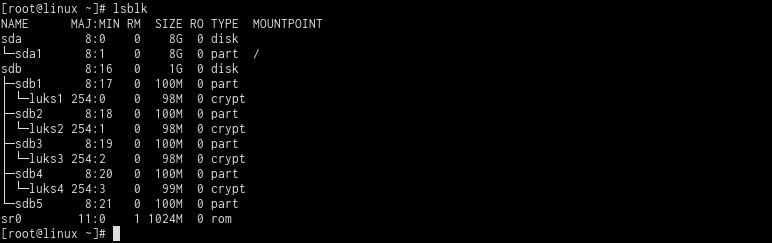
\includegraphics[width=.9\linewidth]{tests/linux_partitions.png}
\caption{\label{fig:linux_partitions}Création des partitions artitions}
\end{figure}

\paragraph{}
Une fois le disque créé, on peut l'ajouter à la machine fonctionnant sous
FreeBSD, qui pourra ainsi directement interagir avec les disques.

\subsection{Tests des différentes fonctionnalités}

\subsubsection{Lecture des métadonnées}
\paragraph{}
Dans un premier temps, afin de tester la lecture de métadonnées sans passer par
les difficultés posées par la lecture de disque (notamment dues à l'emplacement
des métadonnées qui diffère entre \textit{LUKS} et \textit{GELI}), nous avons
créé des fichiers contenant un volume chiffré. Pour ce faire, on crée un fichier
contenant les données d'une des partitions chiffrées \textit{LUKS} réalisées
précédemment à l'aide de la commande \texttt{dd if=/dev/ada1p1 of=file bs=1M}.
Cette opération peut directement être réalisée sur FreeBSD.
\paragraph{}
On tente ensuite d'afficher les métadonnées présentes sur ce fichier. Cela
permet de vérifier que la structure utilisée est cohérente et que les types de
ses variables sont corrects. Pour cela, il d'utiliser les commandes réalisant
cette opérations et de comparer leur sortie sur les deux systèmes.
\paragraph{}
\begin{figure}[h]
\centering
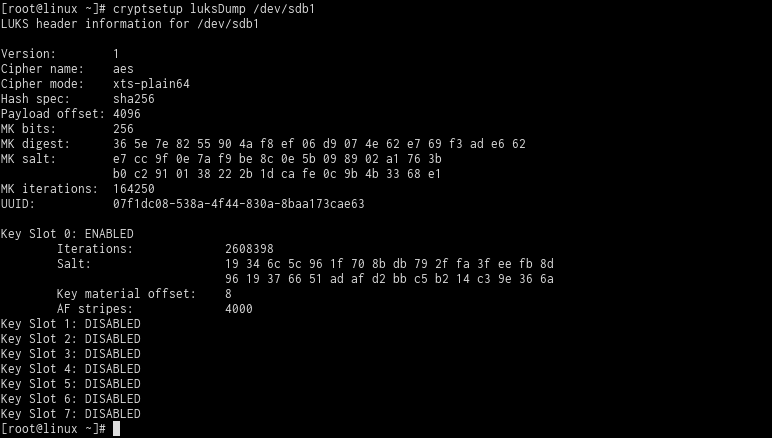
\includegraphics[width=.9\linewidth]{tests/linux_dump_disk.png}
\caption{\label{fig:linux_dump_eli}Affichage des métadonnées sur Linux}
\end{figure}
\paragraph{}
\begin{figure}[h]
\centering
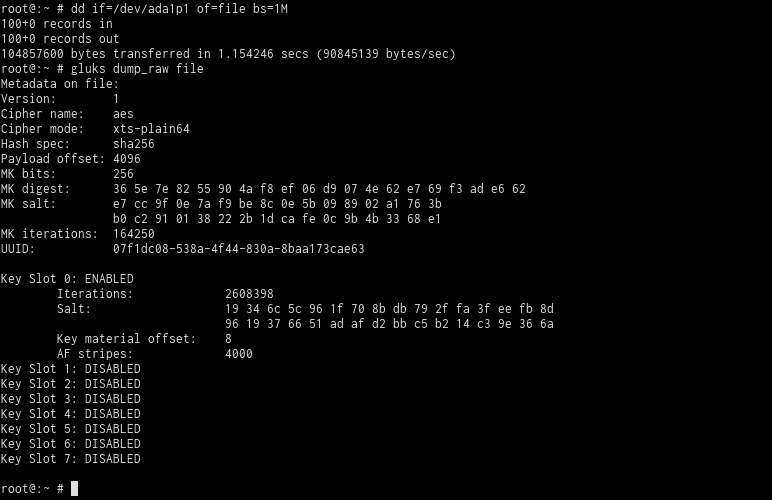
\includegraphics[width=.9\linewidth]{tests/freebsd_dump_file.png}
\caption{\label{fig:freebsd_dump_file}Affichage des métadonnées sur FreeBSD
  depuis un fichier}
\end{figure}

\paragraph{}
Une fois que la structure des métadonnées utilisée a été vérifiée et validée, on
peut poursuivre les tests sur une \textit{vraie} partition chiffrée. Pour ce
faire, on peut utiliser les partitions créées précédemment sous Linux et
accessibles depuis notre système FreeBSD.
\paragraph{}
\begin{figure}[h]
\centering
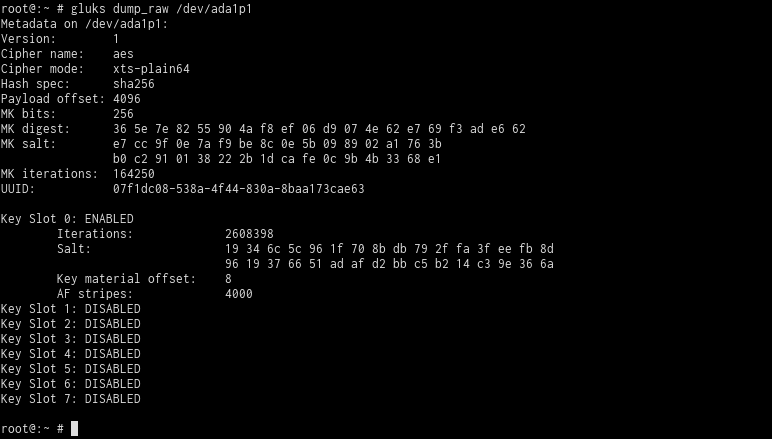
\includegraphics[width=.9\linewidth]{tests/freebsd_dump_disk.png}
\caption{\label{fig:freebsd_dump_disk}Affichage des métadonnées sur FreeBSD
  depuis un disque}
\end{figure}

\subsubsection{Déchiffrement de la clé maître}
\paragraph{}
Pour tester le déchiffrement de la clé maître (ou \textit{masterkey}), on part
de la fonction \texttt{geli attach}, responsable du déchiffrement et de
l'attachement d'un volume chiffré, en enlevant dans un premier dans la partie de
la fonction s'occupant de l'attachement.
\paragraph{}
Sous FreeBSD, l'attachement de volume avec \textit{GELI} consiste premièrement
en son déchiffrement. Une fois déchiffré, un fichier ayant pour extension
\texttt{.eli} (ou \texttt{.luks} dans notre outil) est créé: c'est lui qui
pourra ensuite être monté comme n'importe-quel autre disque. Sur un système
Linux, ce fichier correspond à celui créé dans \texttt{/dev/mapper/} grâce à
\texttt{cryptsetup luksOpen}. Cette partie là est donc ignorée pour l'instant.
\paragraph{}
Les fonctions réalisant le déchiffrement de la clé maître à partir d'une phrase
secrète permettent de savoir si celle-ci est correcte où non. Il est donc
possible de savoir s'il se fait correctement, sans même avoir besoin de monter
le disque pour vérifier son contenu.
\paragraph{}
\begin{figure}[h]
\centering
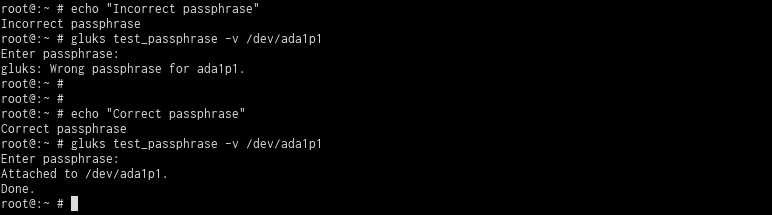
\includegraphics[width=.9\linewidth]{tests/freebsd_test_passphrase.png}
\caption{\label{fig:freebsd_test_passphrase}Test de déchiffrement de la clé maître}
\end{figure}

\subsubsection{Montage et lecture de données}
\paragraph{}
Maintenant qu'il est possible de déchiffrer la clé maître, responsable du
chiffrement du disque, à partir d'une des phrases secrètes, il faut s'assurer du
bon chiffrement du disque en tant que tel.
\paragraph{}
On reprend la fonction précédente pour y ajouter cette fois-ci la partie
responsable de l'attachement du volume chiffré. Après s'être assuré qu'un
fichier en \texttt{.luks} est bien créé dans \texttt{/dev/}, son montage dans
l'arborescence peut se faire. Cette action est réalisée via la commande
\texttt{mount -t ext2fs /dev/ada1p1.luks /mnt}. On peut ensuite s'assurer de son
contenu, en y ayant placé un fichier texte par exemple.

\subsubsection{Montage et écriture de données}
\paragraph{}
De même, une fois le volume déchiffré monté, il doit être possible d'y écrire
des données. On peut par exemple y placer un fichier contenant du texte.
\paragraph{}
Il est ensuite possible de vérifier son contenu depuis notre système Linux, en
ouvrant le disque avec \texttt{cryptsetup} puis en le montant.